\chapter{Acoplamientos Magnéticos y Transformadores}\label{chap.transformadores}

\section{Acoplamientos magnéticos}
\label{sec:acoplamientos}

\subsection{Fundamentos Físicos}
\label{sec:fisica-bobina}

Según la ley de Ampere, una corriente eléctrica circulando por un conductor crea un campo magnético en torno al conductor (\emph{regla de la mano derecha}).

\begin{center}
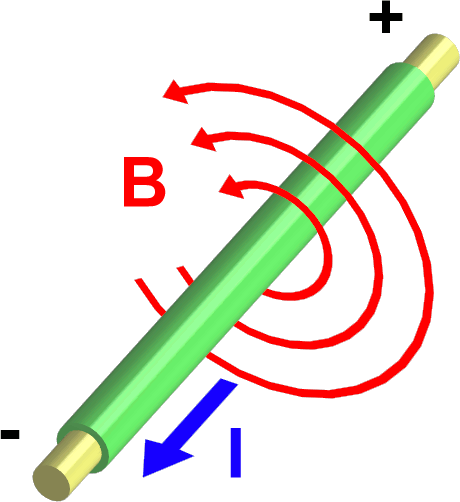
\includegraphics[height=0.2\textheight]{../figs/Electromagnetism.png}
\end{center}

Por otra parte, la ley de Faraday establece que cuando un \emph{campo magnético variable}, $\vec{B}$, atraviesa una espira \emph{estática} aparece una \emph{tensión inducida} \emph{proporcional al flujo} y opuesta a su variación.

\[
u(t) = \frac{\mathrm{d}\phi}{\mathrm{d}t} 
\]
donde $\phi$ es el flujo magnético o cantidad de líneas de fuerza magnética que atraviesan una superficie:

\[
\phi = \vec{B} \cdot \vec{A} \ [\mathrm{Wb}]
\]

\begin{figure}
  \centering
  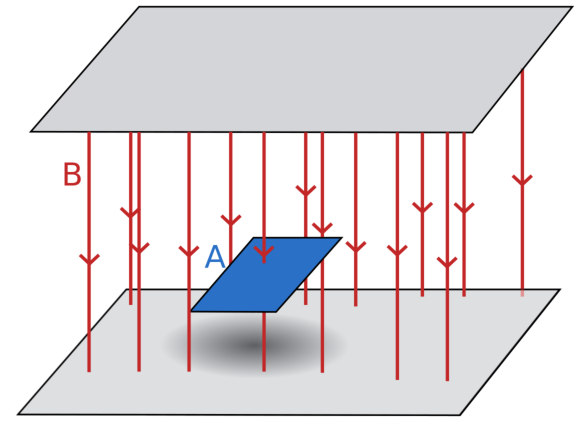
\includegraphics[height=0.2\textheight]{../figs/flujo_magnetico.pdf}
  \caption{Flujo magnético atravesando una superficie.}
  \label{fig:flujo-magnetico}
\end{figure}

Combinando ambas leyes podemos comprender el funcionamiento de la bobina. Una bobina es un arrollamiento de un conductor (\emph{conjunto de $N$ espiras conectadas en serie}) alrededor de un material ferromagnético:
\begin{itemize}
\item Al circular corriente se produce un campo magnético (\emph{ley de Ampere}).
\item Este campo magnético atraviesa la propia bobina y produce una tensión (auto)inducida (\emph{ley de Faraday}).
\end{itemize}

Por tanto, en una bobina de $N$ espiras la tensión autoinducida es:
\[
u(t) = N \cdot \frac{\mathrm{d}\phi(t)}{\mathrm{d} t}
\]

\begin{center}
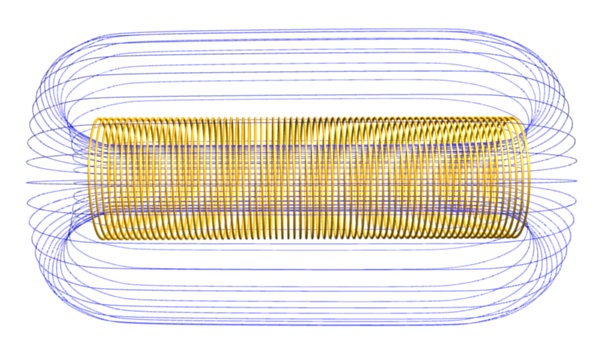
\includegraphics[height=0.2\textheight]{../figs/Solenoide.jpg}
\end{center}

Teniendo en cuenta que en circuito magnético lineal el flujo magnético es proporcional a la corriente:
\[
  \phi(t) = A \cdot i(t) \rightarrow   \frac{\mathrm{d}\phi(t)}{\mathrm{d} i(t)} = \frac{\phi(t)}{i(t)}
\]
podemos obtener la tensión inducida en función de la corriente eléctrica:
\[
u(t) = N \cdot \frac{\mathrm{d}\phi(t)}{\mathrm{d} i(t)} \cdot  \frac{\mathrm{d}i(t)}{\mathrm{d} t} \rightarrow u(t) = N \cdot \frac{\phi(t)}{i(t)} \cdot \frac{\mathrm{d}i(t)}{\mathrm{d} t}
\]
y, en consecuencia, determinamos el coeficiente de autoinductancia, $L \quad [H]$:
\[
  \boxed{L = N \cdot \frac{\phi(t)}{i(t)}}
\]
y la ecuación de la bobina que utilizamos en los circuitos:
\begin{equation}
  \label{eq:bobina-VI}
  \boxed{u(t) = L \cdot \frac{\mathrm{d}i(t)}{\mathrm{d} t}}
\end{equation}

\begin{center}
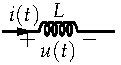
\includegraphics[height=0.1\textheight]{../figs/Bobina.pdf}
\end{center}

\subsection{Acoplamiento magnético}
\label{sec:acoplamiento}

Cuando dos bobinas comparten el núcleo ferromagnético, el flujo magnético producido por cada una de ellas atraviesa a la otra bobina, lo que se conoce como acoplamiento magnético (figura \ref{fig:acoplamiento}).

\begin{figure}
  \centering
  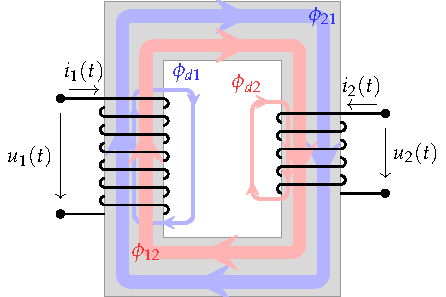
\includegraphics[height=0.2\textheight]{../figs/acoplamientoTikz.pdf}
    \caption{Acoplamiento magnético de dos bobinas. Definición de flujos.}
  \label{fig:acoplamiento}
\end{figure}

En la figura \ref{fig:acoplamiento} se indican los siguientes flujos:
\begin{itemize}
\item   $\phi_{ii}$: flujo producido por la bobina $i$
\item   $\phi_{ij}$: flujo recibido en bobina $i$ producido por bobina $j$
\item   $\phi_{i}$: flujo total que atraviesa la bobina $i$
\item   $\phi_{di}$: flujo de dispersión de la bobina $i$, o flujo que escapa del núcleo y no contribuye al acoplamiento.
\end{itemize}

Estos flujos cumplen las siguientes relaciones:
\begin{align*}
  \phi_{11} &= \phi_{d1} + \phi_{21}\\
  \phi_{1} &= \phi_{11} + \phi_{12}\\
  \phi_{22} &= \phi_{d2} + \phi_{12}\\
  \phi_{2} &= \phi_{22} + \phi_{21}
\end{align*}

La ratio entre el flujo que recibe una bobina y el flujo producido por la bobina emisora se cuantifica con los coeficientes de acoplamiento $k_i$ :
\begin{align}
  \label{eq:coefs-acoplamiento}
  k_1 = \frac{\phi_{21}}{\phi_{11}} = 1 - \frac{\phi_{d1}}{\phi_{11}} \leq 1
  k_2 = \frac{\phi_{12}}{\phi_{22}} = 1 - \frac{\phi_{d2}}{\phi_{22}} \leq 1
\end{align}
Cuando el acoplamiento entre las dos bobinas es perfecto, los flujos de dispersión son nulos y, por tanto:
\[\left.
\begin{array}{cc}
  \phi_{d1} = 0 \rightarrow   \phi_{11} = \phi_{21}\\
  \phi_{d2} = 0 \rightarrow \phi_{22} = \phi_{12} 
  \end{array} \right\} \rightarrow k = 1
\]

A partir de los flujos que recorren el núcleo obtenemos las tensiones inducidas en la bobina 1:
\begin{align*}
  u_1(t) = &N_1 \frac{\mathrm{d}\phi_1}{\mathrm{d}t} = \\
  &N_1 \frac{\mathrm{d}\phi_{11}}{\mathrm{d}t} + N_1 \frac{\mathrm{d}\phi_{12}}{\mathrm{d}t}
\end{align*}
y en la bobina 2:
\begin{align*}
  u_2(t) = &N_2 \frac{\mathrm{d}\phi_2}{\mathrm{d}t} = \\
  &N_2 \frac{\mathrm{d}\phi_{22}}{\mathrm{d}t} + N_2 \frac{\mathrm{d}\phi_{21}}{\mathrm{d}t}
\end{align*}

En estas ecuaciones podemos identificar los términos debidos a la autoinducción, con sus dos coeficientes de autoinducción:
\begin{align}
  \label{eq:acoplamiento-autoinduccion}
  L_1 &= N_1 \frac{\phi_{11}}{i_1}\\
  L_2 &= N_2 \frac{\phi_{22}}{i_2}
\end{align}
y los términos de inducción mutua, con los que podemos definir los coeficientes de inducción mutua, $M_{12}$ y $M_{21}$:
\begin{align}
  \label{eq:coef-induccion-mutua}
  M_{12} &= N_1 \frac{\phi_{12}}{i_2}\\
  M_{21} &= N_2 \frac{\phi_{21}}{i_1}
\end{align}

Los coeficientes de acoplamiento y los coeficientes de inducción mutua son iguales cuando el circuito magnético es lineal:
  \begin{align*}
  M_{12} = M_{21} &= M\\
  k_1 = k_2 &= k    
  \end{align*}
  Esta condición nos permite relacionar los coeficientes de autoinducción con el coeficiente de inducción mutua:
  \begin{equation}
    \label{eq:L-M}
    \boxed{M = k \sqrt{L_1 \cdot L_2}} \qquad  k \leq 1
  \end{equation}

  \subsection{Representación Circuital}
  \label{sec:org1754ad3}
  Para representar un acoplamiento magnético en un circuito eléctrico
  se emplea la convención del punto, señalando con un punto los
  terminales de las bobinas por los que hay que introducir corrientes
  que producen flujos del mismo sentido. Una corriente que entra por
  un terminal con punto induce una tensión positiva en el otro
  terminal con punto.

  En la siguiente figura, las dos bobinas están arrolladas de forma
  que introduciendo corrientes por los terminales superiores se
  obtienen flujos que circulan en el mismo sentido:
  \begin{center}
    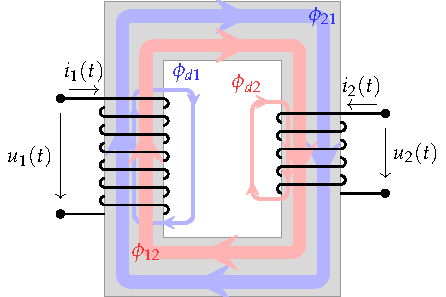
\includegraphics[height=0.2\textheight]{../figs/acoplamientoTikz.pdf}
  \end{center}

\begin{center}
  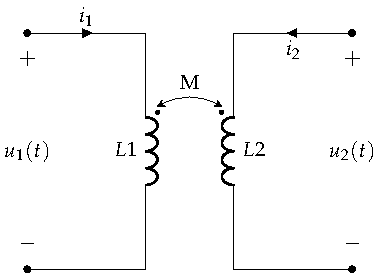
\includegraphics[height=0.2\textheight]{../figs/acoplamiento_circuito.pdf}
\end{center}

Las ecuaciones circuitales de este acoplamiento son:
\begin{align*}
  u_1(t) &= L_1 \frac{\mathrm{d}i_1(t)}{\mathrm{d}t} + M \frac{\mathrm{d}i_2(t)}{\mathrm{d}t}\\
  u_2(t) &= M \frac{\mathrm{d}i_1(t)}{\mathrm{d}t} + L_2 \frac{\mathrm{d}i_2(t)}{\mathrm{d}t}
\end{align*}

Por el contrario, la siguiente figura representa un acoplamiento en el
que las bobinas están arrolladas de forma que los flujos tienen
sentidos contrapuestos si se introduce corriente por los terminales
superiores.

\begin{center}
  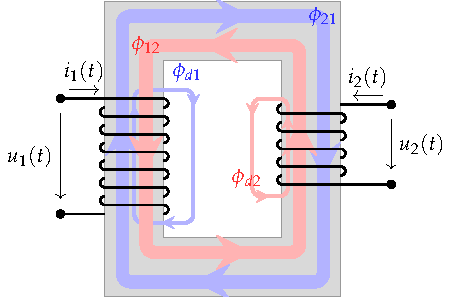
\includegraphics[height=0.2\textheight]{../figs/acoplamientoTikz_opuesto.pdf}
\end{center}
\begin{center}
  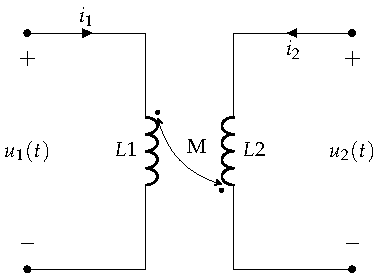
\includegraphics[height=0.2\textheight]{../figs/acoplamiento_circuito_opuesto.pdf}
\end{center}

Las ecuaciones circuitales de este acoplamiento son:

\begin{align*}
  u_1(t) &= L_1 \frac{\mathrm{d}i_1(t)}{\mathrm{d}t} - M \frac{\mathrm{d}i_2(t)}{\mathrm{d}t}\\
  u_2(t) &= - M \frac{\mathrm{d}i_1(t)}{\mathrm{d}t} + L_2 \frac{\mathrm{d}i_2(t)}{\mathrm{d}t}
\end{align*}

Las ecuaciones anteriores están expresadas en el dominio del
tiempo. Cuando las bobinas están alimentadas por corriente alterna
sinusoidal, podemos expresar las ecuaciones con fasores, ya sea para
flujos en el mismo sentido:
\begin{align*}
  \overline{U}_1 &= j \omega L_1 \overline{I}_1 + j \omega M \overline{I}_2\\
  \overline{U}_2 &= j \omega M \overline{I}_1 + j \omega L_2 \overline{I}_2
\end{align*}
o para flujos contrapuestos:
\begin{align*}
  \overline{U}_1 &= j \omega L_1 \overline{I}_1 - j \omega M \overline{I}_2\\
  \overline{U}_2 &= - j \omega M \overline{I}_1 + j \omega L_2 \overline{I}_2
\end{align*}


Como ejemplo, calculemos la bobina equivalente de dos bobinas
conectadas en serie. Cuando las bobinas están acopladas con flujos en
el mismo sentido (figura \ref{fig:bobinas-serie-mismo-sentido}), las
ecuaciones son:

\begin{figure}
  \centering
  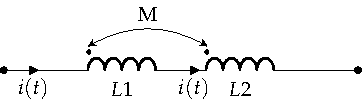
\includegraphics[height=0.1\textheight]{../figs/bobinas_serie.pdf}
  \caption{Dos bobinas conectadas en serie con acoplamiento magnético
    con flujos en el mismo sentido.}
  \label{fig:bobinas-serie-mismo-sentido}
\end{figure}

  \begin{align*}
    \overline{U}_1 &= (j \omega L_1 + j \omega M) \overline{I}\\
    \overline{U}_2 &= (j \omega L_2 + j \omega M) \overline{I}\\
    \overline{U} &= \overline{U}_1 + \overline{U}_2 
  \end{align*}
  que permiten obtener la equivalencia de la ecuación
  \ref{eq:bobinas-serie-mismo-sentido}:
  \begin{equation}
    \label{eq:bobinas-serie-mismo-sentido}
    L = L_1 + L_2 + 2M
  \end{equation}

  Sin embargo, si las bobinas están acopladas con flujos contrapuestos
  (figura \ref{fig:bobinas-serie-flujo-contrapuesto}), las ecuaciones
  son:
  \begin{figure}
    \centering
    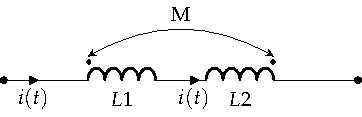
\includegraphics[height=0.1\textheight]{../figs/bobinas_serie_opuesto.pdf}
    \caption{Dos bobinas conectadas en serie con acoplamiento
      magnético con flujos contrapuestos.}
    \label{fig:bobinas-serie-flujo-contrapuesto}
  \end{figure}

\begin{align*}
  \overline{U}_1 &= (j \omega L_1 - j \omega M) \overline{I}\\
  \overline{U}_2 &= (j \omega L_2 - j \omega M) \overline{I}\\
  \overline{U} &= \overline{U}_1 + \overline{U}_2 
\end{align*}
de forma que la inductancia equivalente es ahora:
\begin{equation}
  \label{eq:bobinas-serie-contrapuesto}
  L = L_1 + L_2 - 2M
\end{equation}

\section{Transformadores}
\label{sec:transformadores}

Un transformador es una máquina eléctrica compuesta por dos o más
devanados arrollados sobre un núcleo ferromagnético sin conexión
eléctrica entre los devanados (figura \ref{fig:acoplamiento}), de
forma que la transmisión de energía se realiza únicamente mediante el
acoplamiento magnético.

\subsection{Transformador Real}
\label{sec:transformador-real}

La figura \ref{fig:trafo-real} es la representación circuital
simplificada de un transformador real, es decir, un transformador que
tiene pérdidas resistivas en las bobinas y cuyo acoplamiento magnético
no es perfecto ($k < 1$).

\begin{figure}
  \centering
  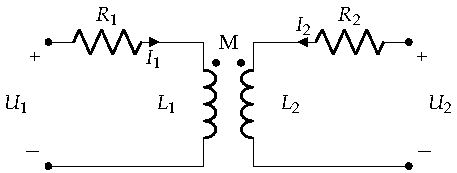
\includegraphics[height=0.2\textheight]{../figs/Trafo_Real.pdf}
  \caption{Representación circuital de un transformador real}
  \label{fig:trafo-real}
\end{figure}
Las ecuaciones de este transformador son:
\begin{align}
  \label{eq:trafo-real}
  \overline{U}_1 &= (R_1 + j \omega L_1) \cdot \overline{I}_1 + j \omega M \cdot\overline{I}_2\\
  \overline{U}_2 &= j \omega M \cdot \overline{I}_1 + (R_2 + j \omega L_2) \cdot \overline{I}_2
\end{align}

En general, los terminales de la izquierda ($U_1$) se denominan como
primario, y los terminales de la derecha ($U_2$) como secundario.

Supongamos que conectamos una impedancia en el secundario de este
transformador. Para calcular la impedancia que se ve desde el primario
debemos calcular la relación $\overline{U}_1/\overline{I}_1$ a partir
de las ecuaciones \ref{eq:trafo-real} y de la ecuación de la
impedancia:

\begin{equation*}
  \overline{U}_2 = - \overline{I}_2 \cdot \overline{Z}_L
\end{equation*}

\begin{figure}
  \centering
  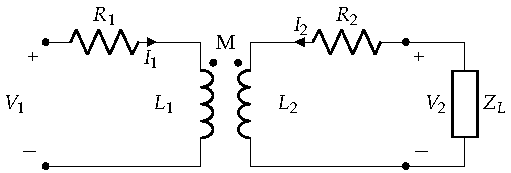
\includegraphics[height=0.2\textheight]{../figs/Trafo_Real_ImpSec.pdf}
  \caption{Impedancia conectada en el secundario de un transformador
    real.}
  \label{fig:trafo-real-impedancia-secundario}
\end{figure}


Combinando la ecuación del secundario con la ecuación de la carga
obtenemos la corriente en el secundario:
\[
  \overline{I}_2 = - \frac{j \omega M}{(R_2 + j \omega L_2) +
    \overline{Z}_L} \cdot \overline{I}_1
\]
que podemos insertar en la ecuación del primario para obtener la
impedancia de entrada:

\begin{equation}
  \label{eq:trafo-real-impedancia-entrada}
  \overline{Z}_{in}  = \frac{\overline{U}_1}{\overline{I}_1} =  (R_1 + j \omega L_1) + \frac{\omega^2 M^2}{(R_2 + j \omega L_2) + \overline{Z}_L} = \boxed{\overline{Z}_1 + \frac{\omega^2 M^2}{\overline{Z}_2 + \overline{Z}_L}}
\end{equation}
Podemos interpretar este resultado como la conexión serie de la
impedancia de primario con una impedancia transformada, obtenida a
partir de la conexión serie de la impedancia de secundario y la
impedancia de carga.

Calculemos ahora el equivalente de Thévenin desde secundario de una
fuente real conectada en el primario (figura
\ref{fig:trafo-real-fuente-primario}).

\begin{figure}
  \centering
  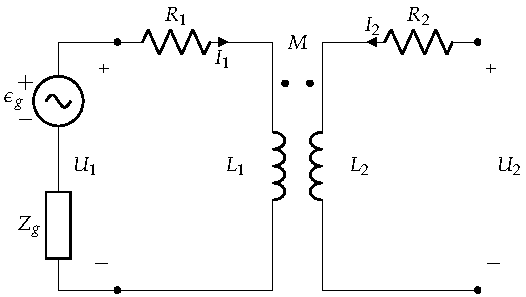
\includegraphics[height=0.2\textheight]{../figs/Trafo_Real_FuentePrimario.pdf}
  \caption{Fuente real conectada en el primario de un transformador
    real.}
  \label{fig:trafo-real-fuente-primario}
\end{figure}

La ecuación del generador es:
\[
  \overline{U}_1 = \overline{\epsilon}_g - \overline{I}_1 \cdot
  \overline{Z}_g
\]
mientras que las ecuaciones del transformador se simplifican al tener
en cuenta que $\overline{I}_2 = 0$:
\begin{align*}
  \overline{U}_1 &= (R_1 + j \omega L_1) \cdot \overline{I}_1\\
  \overline{U}_2 &= j \omega M \cdot \overline{I}_1
\end{align*}
Despejamos la corriente de primario $I_1$:
\[
  \overline{I}_1 = \frac{\overline{\epsilon_g}}{\overline{Z}_1 +
    \overline{Z}_g}
\]
y la utilizamos en la ecuación del secundario para obtener la tensión
de Thévenin:

\begin{equation}
  \label{eq:trafo-real-tension-thevenin}
  \overline{U}_2 = \boxed{\overline{\epsilon}_{th} = \frac{j\omega M}{\overline{Z}_1 + \overline{Z}_g} \cdot \overline{\epsilon}_g}
\end{equation}
Este resultado recuerda a la expresión de un divisor de tensión,
aunque el numerador está transformado respecto a la expresión
original.

Para calcular la impedancia de Thévenin apagamos la fuente
$\epsilon_g$ y conectamos una fuente de prueba en secundario (figura
\ref{fig:trafo-real-impedancia-thevenin}).
\begin{figure}
  \centering
  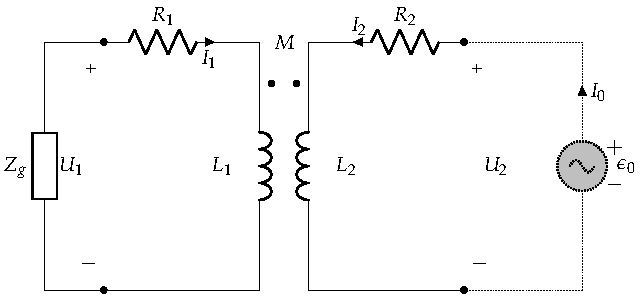
\includegraphics[height=.2\textheight]{../figs/Trafo_Real_ImpedanciaPrimario.pdf}
  \caption{Cálculo de la impedancia de Thévenin de una fuente
    conectada en primario.}
  \label{fig:trafo-real-impedancia-thevenin}
\end{figure}
Con esta conexión, las ecuaciones del transformador son:
\begin{align*}
  \overline{U}_1 &= (R_1 + j \omega L_1) \cdot \overline{I}_1 + j \omega M \cdot\overline{I}_0\\
  \overline{\epsilon}_0 &= j \omega M \cdot \overline{I}_1 + (R_2 + j \omega L_2) \cdot \overline{I}_0
\end{align*}
y la ecuación de la impedancia:
\[
  \overline{U}_1 = - \overline{Z}_g \cdot \overline{I}_1
\]
Combinando estas ecuaciones obtenemos la impedancia de Thévenin:

\begin{equation}
  \label{eq:trafo-real-impedancia-thevenin}
  \boxed{\overline{Z}_{th} = \frac{\overline{\epsilon}_0}{\overline{I}_0} = \overline{Z}_2 + \frac{\omega^2 M^2}{\overline{Z}_1 + \overline{Z}_g}}
\end{equation}
Esta expresión, al igual que la ecuación
\ref{eq:trafo-real-impedancia-entrada}, se asemeja a la conexión serie
de la impedancia de secundario con una impedancia transformada
obtenida a partir de la impedancia de primario y del generador.

\subsection{Transformador Perfecto}
\label{sec:trafo-perfecto}

Para facilitar el tratamiento circuital de un transformador, emplearemos el modelo del transformador perfecto (figura \ref{fig:trafo-perfecto}), que incluye dos simplificaciones:
\begin{itemize}
\item Las pérdidas resistivas son despreciables.
  \[
    R_1 = R_2 = 0
  \]
\item El acoplamiento es perfecto.
  \[
    k = 1 \rightarrow \left\{
      \begin{array}{cc}
        \phi_{12} &= \phi_{22}\\
        \phi_{21} &= \phi_{11}\\
      \end{array} \right.
  \]
\end{itemize}

\begin{figure}
  \centering
  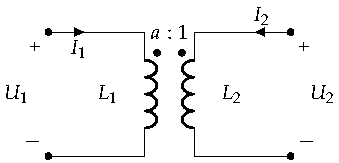
\includegraphics[height=0.15\textheight]{../figs/Trafo_Perfecto.pdf}
  \caption{Representación circuital de un transformador perfecto.}
  \label{fig:trafo-perfecto}
\end{figure}

Las ecuaciones de este modelo de transformador son:
\begin{align*}
  \overline{U}_1 &= j \omega L_1 \cdot \overline{I}_1 + j \omega M \cdot \overline{I}_2\\
  \overline{U}_2 &= j \omega M \cdot \overline{I}_1 + j \omega L_2 \cdot \overline{I}_2
\end{align*}

Teniendo en cuenta que $k = 1$, a partir de las ecuaciones de
$M_{12} = M_{21} = M$:
\[
  N_1 \frac{\phi_{12}}{i_2} = N_2 \frac{\phi_{21}}{i_1}
\]
podemos escribir:
\[
  N_1 \frac{\phi_{22}}{i_2} = N_2 \frac{\phi_{11}}{i_1}
\]
Además, con las definiciones de $L_1$ y $L_2$:
\[
  N_1 \frac{L_2}{N_2} = N_2 \frac{L_1}{N_1}
\]
obtenemos la relación de transformación de un transformador perfecto:
\begin{equation}
  \label{eq:trafo-perfecto-a}
  \boxed{\frac{L_1}{L_2} = \left(\frac{N_1}{N_2}\right)^2 = a^2}
\end{equation}


Con esta relación de transformación podemos simplificar las ecuaciones
del transformador. En primer lugar dividimos las ecuaciones:
\[
  \frac{\overline{U}_1}{\overline{U}_2} = \frac{j \omega L_1 \cdot
    \overline{I}_1 + j \omega M \cdot \overline{I}_2}{j \omega M \cdot
    \overline{I}_1 + j \omega L_2 \cdot \overline{I}_2}
\]
y empleamos la relación de transformación:
\[
  \frac{L_1}{L_2} = a^2 \rightarrow \left\{
    \begin{array}{ll}
      L_1 &= a^2 \cdot L_2\\
      M &= a \cdot L_2\\
    \end{array}\right.
\]
para escribir:
\[
  \frac{\overline{U}_1}{\overline{U}_2} = \frac{a^2 L_2 \cdot
    \overline{I}_1 + a L_2 \cdot \overline{I}_2}{a L_2 \cdot
    \overline{I}_1 + L_2 \cdot \overline{I}_2}
\]
que, después de simplificar, conduce a la relación entre tensiones de
un transformador perfecto:
\begin{equation}
  \label{eq:trafo-perfecto-tensiones}
  \boxed{\frac{\overline{U}_1}{\overline{U}_2} = a = \frac{N_1}{N_2}}
\end{equation}

Estas relaciones nos permiten simplificar los resultados obtenidos con
el transformador real. En primer lugar, la impedancia de entrada en un
transformador real con $R_1 = R_2 = 0$ es:

\[
  \overline{Z}_{in} = j\omega L_1 + \frac{\omega^2 M^2}{j\omega L_2 +
    \overline{Z}_L}
\]

\begin{figure}
  \centering
  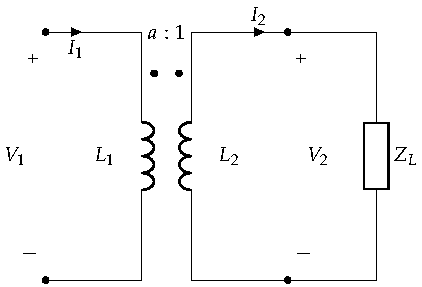
\includegraphics[height=0.2\textheight]{../figs/TrafoPerfecto_ImpedanciaSecundario.pdf}
  \caption{Impedancia conectada en el secundario de un transformador perfecto.}
  \label{fig:trafo-perfecto-impedancia-secundario}
\end{figure}

A continuación, teniendo en cuenta la relación entre $L_1$, $L_2$ y
$M$:
\[
  \overline{Z}_{in} = j\omega L_1 + \frac{\omega^2 M^2}{j\omega L_2 +
    \overline{Z}_L} = \frac{j\omega L_1 \overline{Z}_L}{j\omega L_2 +
    \overline{Z}_L}
\]
y, finalmente, incorporando la relación de transformación:
\begin{equation}
  \label{eq:trafo-perfecto-impedancia-entrada}
  \overline{Z}_{in} =  a^2 \cdot \frac{j \omega L_2 \cdot \overline{Z}_L}{j\omega L_2 + \overline{Z}_L} =  \frac{j \omega L_1 \cdot a^2 \cdot \overline{Z}_L}{j\omega L_1 + a^2 \cdot \overline{Z}_L}
\end{equation}
Esta expresión se puede interpretar como un factor de escala aplicado
a una conexión en paralelo entre la inductancia de secundario y la
impedancia de carga, o como una conexión en paralelo entre la
inductancia de primario y la impedancia de carga con un factor de
escala.

De forma equivalente, el equivalente de Thévenin de una fuente real
conectada en primario es:

\[
  \overline{\epsilon}_{th} = \overline{U}_2 = \frac{j\omega M}{j\omega
    L_1 + \overline{Z}_g} \cdot \overline{\epsilon}_g
\]

\begin{figure}
  \centering
  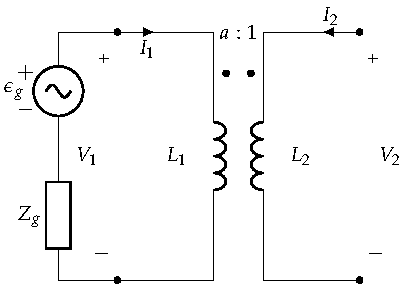
\includegraphics[height=0.2\textheight]{../figs/Trafo_Perfecto_FuentePrimario.pdf}
  \caption{Fuente real conectada en el primario de un transformador perfecto.}
  \label{fig:trafo-perfecto-fuente-primario}
\end{figure}
Teniendo en cuenta que $M = L_1/a$:

\begin{equation}
  \label{eq:trafo-perfecto-tension-thevenin}
  \overline{\epsilon}_{th} = \frac{1}{a} \cdot \left(\frac{j\omega
      L_1}{j\omega L_1 + \overline{Z}_g}\right) \cdot
  \overline{\epsilon}_g
\end{equation}

Esta expresión corresponde a un divisor de tensión entre la impedancia
del generador y la inductancia del primario, aplicando previamente un
factor de escala.

Por otra parte, la impedancia de Thévenin es:
\[
  \overline{Z}_{th} = j\omega L_2 + \frac{\omega^2 M^2}{j\omega L_1 +
    \overline{Z}_g}
\]
Aplicando las relaciones $L_2 = L_1/a^2$ y $M = L_1/a$ obtenemos:
\begin{equation}
  \label{eq:trafo-perfecto-impedancia-thevenin}
  \overline{Z}_{th} = \frac{1}{a^2} \cdot \frac{j \omega L_1 \cdot \overline{Z}_g}{j\omega L_1 + \overline{Z}_g}
\end{equation}
Este resultado se puede interpretar como una impedancia equivalente de
una conexión en paralelo entre la inductancia de primario y la
impedancia del generador, aplicando previamente un factor de escala.


\subsection{Transformador Ideal}
\label{sec:trafo-ideal}

Como siguiente y último paso en la simplificación del circuito que
representa un transformador, vamos a considerar el transformador ideal
(figura \ref{fig:trafo-ideal}). Este modelo de transformador comparte
con el transformador perfecto las dos condiciones ya conocidas (las
pérdidas resistivas son despreciables, y el acoplamiento es perfecto)
y añade una adicional: las bobinas tienen un número muy elevado de
espiras.
  \begin{align*}
  N_1 &\to \infty\\
  N_2 &\to \infty
  \end{align*}

  \begin{figure}
    \centering
    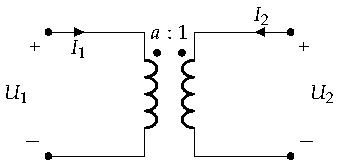
\includegraphics[height=0.15\textheight]{../figs/Trafo_Ideal.pdf}
    \caption{Representación circuital de un transformador ideal.}
    \label{fig:trafo-ideal}
  \end{figure}

  Teniendo en cuenta la relación que la tensión tiene con el número de espiras, este modelo implica que los flujos fasoriales que atraviesan las bobinas deben ser nulos:

  \begin{align*}
  \overline{U}_1 &= N_1 \overline{\phi}_1 \rightarrow \overline{\phi}_1 \to 0\\
  \overline{U}_2 &= N_2 \overline{\phi}_2 \rightarrow \overline{\phi}_2 \to 0\\
\end{align*}
donde
\begin{align*}
  \overline{\phi}_1 &= \overline{\phi}_{11} + \overline{\phi}_{12}\\
  \overline{\phi}_2 &= \overline{\phi}_{22} + \overline{\phi}_{21}
\end{align*}

Teniendo en cuenta que el acoplamiento es perfecto, $k = 1$:
  \[
    \left.
      \begin{array}{ll}
      \phi_{12} &= \phi_{22}\\
      \phi_{21} &= \phi_{11}\\
    \end{array} \right\} 
       \rightarrow
       \left\{
    \begin{array}{ll}
      0 &= \overline{\phi}_{21} + \overline{\phi}_{12}\\
      0 &= \overline{\phi}_{12} + \overline{\phi}_{21}\\
    \end{array}\right.
\]
y, por tanto,
\[
  \overline{\phi}_{11} + \overline{\phi}_{22} = 0
\]

Recuperando las definiciones de $L_1$, $L_2$:
  \[
    L_1 = N_1 \frac{\phi_{11}}{I_1}; \quad L_2 = N_2
    \frac{\phi_{22}}{I_2}
  \]
podemos escribir:
\[
  \frac{L_1 \overline{I}_1}{N_1} + \frac{L_2 \overline{I}_2}{N_2}
  = 0
\]
y, a continuación,
\[
    L_1 = L_2 \cdot \left(\frac{N_1}{N_2}\right)^2 \rightarrow
    \frac{N_1L_2 \overline{I}_1}{N^2_2} + \frac{L_2
      \overline{I}_2}{N_2} = 0
  \]
Por tanto, en un transformador ideal, las corrientes en primario y secundario están relacionadas mediante la expresión \ref{eq:trafo-ideal-corrientes}:
\begin{equation}
  \label{eq:trafo-ideal-corrientes}
  \boxed{\frac{\overline{I}_1}{\overline{I}_2} = \mp \frac{1}{a} =
    \mp \frac{N_2}{N_1}}
\end{equation}
En esta ecuación, si las dos corrientes van en el mismo sentido ($I_1$ entrando en primario e $I_2$ saliendo de secundario), la ecuación tendrá un signo positivo.

Esta relación, unida a la relación de tensiones que obtuvimos en el modelo de transformador perfecto, (ecuación \ref{eq:trafo-perfecto-tensiones}), nos permite calcular el triángulo de potencias en primario y secundario, y la relación entre ambos:
\[
  \overline{S}_2 = \overline{U}_2 \cdot (-\overline{I}_2)^* = \frac{1}{a} \cdot
  \overline{U}_1 \cdot a \cdot \overline{I}_1^* = \overline{S}_1
  \]
En esta ecuación aplicamos un signo negativo a la corriente $I_2$ dado su sentido en la figura \ref{fig:trafo-ideal}. Así pues, un transformador ideal no consume ni potencia activa ni potencia reactiva (ecuación \ref{eq:trafo-ideal-potencias}):
\begin{equation}
  \label{eq:trafo-ideal-potencias}
  \boxed{\overline{S}_1 = \overline{S}_2} \quad \boxed{P_1 = P_2}
  \quad \boxed{Q_1 = Q_2}
  \end{equation}

  \subsubsection{Transferencia de Circuitos}
\label{sec:transferencia-circuitos}

El modelo de transformador ideal permite transferir circuitos de primario a secundario y viceversa de forma sencilla. A continuación, las figuras de la izquierda representan los circuitos con transformador ideal, y las de la derecha el circuito equivalente sin transformador una vez realizada la transferencia. Todos los transformadores de estos circuitos tienen los puntos en concordancia y las corrientes en el mismo sentido. En consecuencia, los signos de todas las ecuaciones son positivos. En caso contrario, habrá que adaptar los signos como corresponda.  

\begin{itemize}
\item Fuente de tensión ideal de secundario a primario
  \begin{center}
    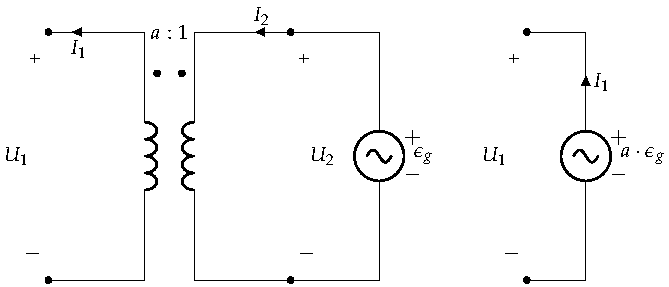
\includegraphics[height=.2\textheight]{../figs/TrafoIdeal_VSec.pdf}
  \end{center}

  \[
    \overline{U}_1 = a \cdot \overline{U}_2 \rightarrow
    \boxed{\overline{\epsilon}_{g1} = a \cdot \overline{\epsilon}_g}
  \]
\item Fuente de Tensión de primario a secundario
  \begin{center}
    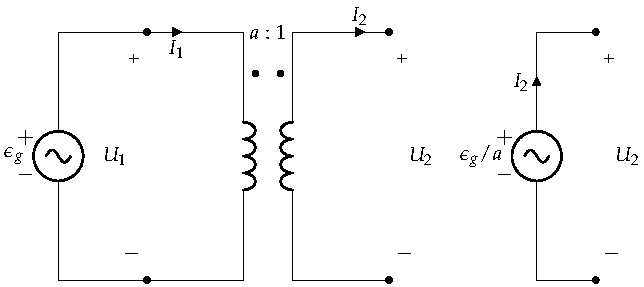
\includegraphics[height=.2\textheight]{../figs/TrafoIdeal_VPrim.pdf}
  \end{center}

  \[
    \overline{U}_2 = \overline{U}_1 / a \rightarrow
    \boxed{\overline{\epsilon}_{g2} = \overline{\epsilon}_g / a}
  \]
\item Fuente de corriente de secundario a primario
  \begin{center}
    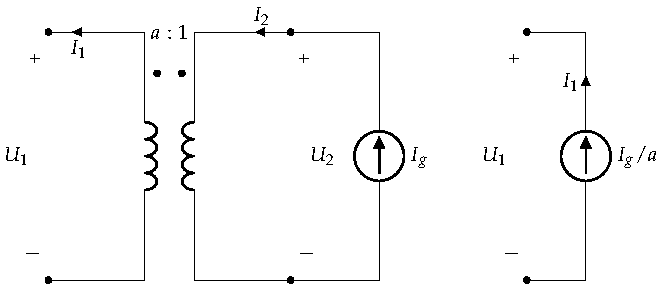
\includegraphics[height=.2\textheight]{../figs/TrafoIdeal_ISec.pdf}
  \end{center}

  \[
    \overline{I}_1 = \overline{I}_2 / a \rightarrow
    \boxed{\overline{I}_{g1} = \overline{I}_g / a}
  \]
\item Fuente de corriente de primario a secundario
  \begin{center}
    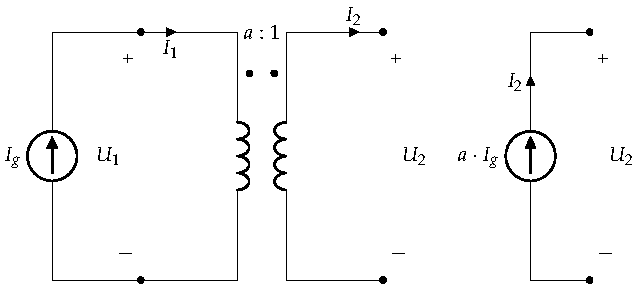
\includegraphics[height=.2\textheight]{../figs/TrafoIdeal_IPrim.pdf}
  \end{center}
  \[
    \overline{I}_2 = a \cdot \overline{I}_1 \rightarrow
    \boxed{\overline{I}_{g2} = a \cdot \overline{I}_g}
  \]
\item Impedancia de secundario a primario
  \begin{center}
    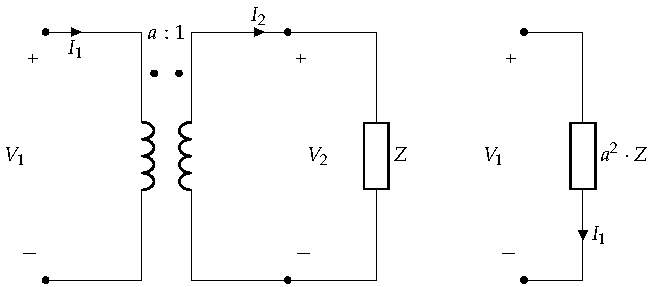
\includegraphics[height=.2\textheight]{../figs/TrafoIdeal_ZSec.pdf}
  \end{center}
  \[
    \left.
      \begin{array}{ll}
        \overline{U}_1 &= a \cdot \overline{U}_2\\
        \overline{I}_1 &= \overline{I}_2 / a\\
      \end{array}\right\}
    \rightarrow \boxed{\overline{Z}_1 =
      \frac{\overline{U}_1}{\overline{I}_1} = a^2 \cdot \overline{Z}}
  \]
\item Impedancia de primario a secundario
  \begin{center}
    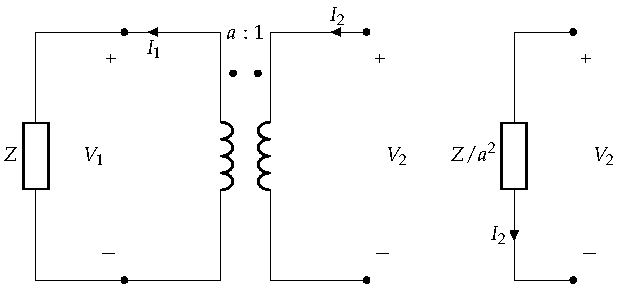
\includegraphics[height=.2\textheight]{../figs/TrafoIdeal_ZPrim.pdf}
  \end{center}
  \[
    \left.
      \begin{array}{ll}
        \overline{U}_2 &= \overline{U}_1 /a\\
        \overline{I}_2 &= a \cdot \overline{I}_1\\
      \end{array}\right\}
    \rightarrow \boxed{\overline{Z}_2 =
      \frac{\overline{U}_2}{\overline{I}_2} = \overline{Z} / a^2}
  \]
\end{itemize}

\subsection{Transformador Perfecto y Transformador Ideal}
\label{sec:perfecto-vs-ideal}

En la ecuación \ref{eq:trafo-perfecto-impedancia-entrada} obteníamos dos expresiones para la impedancia de entrada vista desde el primario de un transformador perfecto. Teniendo en cuenta cómo realizar transferencia de circuitos con un transformador ideal, podemos volver a interpretar estas dos expresiones.

La primera expresión es la impedancia equivalente de una inductancia $L_1$ en paralelo con una impedancia $Z_L$ transferida de secundario a primario de un transformador ideal. Tal y como se ve en la figura \ref{fig:trafo-perfecto-ideal-L1}, esta expresión permite sustituir el transformador perfecto por un transformador ideal en paralelo con la inductancia de primario.
  \[
    \overline{Z}_{in} = \frac{j \omega L_1 \cdot (a^2
    \overline{Z}_L)}{j\omega L_1 + (a^2 \cdot \overline{Z}_L)}
  \]
  \begin{figure}
    \centering
    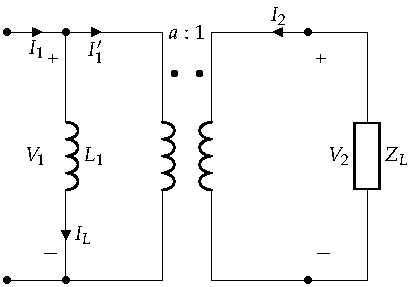
\includegraphics[height=.2\textheight]{../figs/TrafoPerfecto_Ideal.pdf}
    
    \caption{Circuito equivalente de un transformador perfecto con una impedancia de carga usando un transformador ideal y la inductancia de primario.}
    \label{fig:trafo-perfecto-ideal-L1}
  \end{figure}

  La segunda expresión es la impedancia equivalente de una inductancia $L_2$ transferida de secundario a primario de un transformador ideal en paralelo con una impedancia $Z_L$. Tal y como se ve en la figura \ref{fig:trafo-perfecto-ideal-L2}, esta expresión permite sustituir el transformador perfecto por un transformador ideal en paralelo con la inductancia de secundario.
  \[
    \overline{Z}_{in} = a^2 \cdot \frac{j \omega L_2 \cdot
    \overline{Z}_L}{j\omega L_2 + \overline{Z}_L}
\]

  \begin{figure}
    \centering
    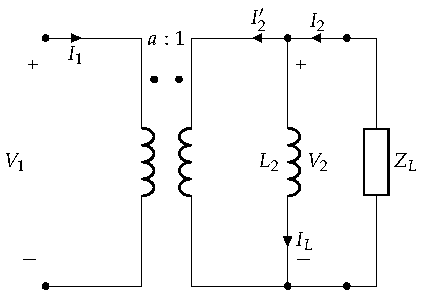
\includegraphics[height=.2\textheight]{../figs/TrafoPerfecto_Ideal2.pdf}
        \caption{Circuito equivalente de un transformador perfecto con una impedancia de carga usando un transformador perfecto empleando la inductancia de primario.
}
\label{fig:trafo-perfecto-ideal-L2}
  \end{figure}

  Este mismo razonamiento puede aplicarse a transformadores perfectos con fuentes de tensión en primario (figura \ref{fig:trafo-perfecto-ideal-V1}), cuyas expresiones se recogían en las ecuaciones \ref{eq:trafo-perfecto-impedancia-thevenin} y \ref{eq:trafo-perfecto-tension-thevenin}:
  \[
    \overline{Z}_{th} = \frac{1}{a^2} \cdot \frac{j \omega L_1 \cdot
    \overline{Z}_g}{j\omega L_1 + \overline{Z}_g}
  \]

  \[
    \overline{\epsilon}_{th} = \frac{1}{a} \cdot \left(\frac{j\omega
      L_1}{j\omega L_1 + \overline{Z}_g}\right) \cdot
    \overline{\epsilon}_g
  \]

  \begin{figure}
    \centering
    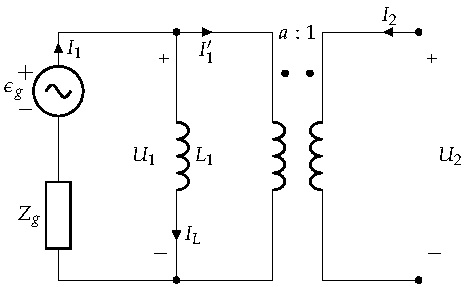
\includegraphics[height=0.2\textheight]{../figs/TrafoPerfecto_Ideal_FuentePrim.pdf}
    \caption{Circuito equivalente de un transformador perfecto con una fuente de tensión conectada en primario}
    \label{fig:trafo-perfecto-ideal-V1}
  \end{figure}

  En estos ejemplos, observamos que podemos sustituir un transformador perfecto por un transformador ideal en paralelo con una de sus dos inductancias, bien en primario o bien en secundario, según convenga a los propósitos del circuito.

  Resolvamos otro ejemplo aplicando estas observaciones, una fuente de tensión real conectada en secundario (\ref{fig:trafo-perfecto-ideal-V2}). La impedancia equivalente será:
  \[
    \overline{Z}_{th} = a^2 \cdot \frac{j \omega L_2 \cdot
    \overline{Z}_g}{j\omega L_2 + \overline{Z}_g}
  \]
mientras que la tensión de Thévenin es:
  \[
    \overline{\epsilon}_{th} = a \cdot \left(\frac{j\omega
      L_2}{j\omega L_2 + \overline{Z}_g}\right) \cdot
    \overline{\epsilon}_g
  \]

  \begin{figure}
    \centering
    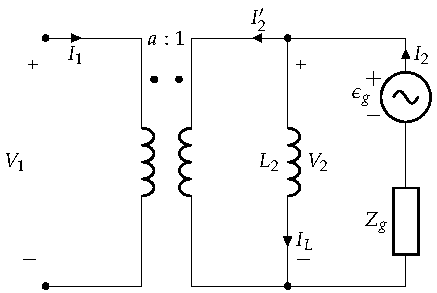
\includegraphics[height=0.2\textheight]{../figs/TrafoPerfecto_Ideal_FuenteSec.pdf}
    \caption{Circuito equivalente de un transformador perfecto con una fuente de tensión conectada en secundario.}
    \label{fig:trafo-perfecto-ideal-V2}
  \end{figure}

  
\subsection{Transformador de Varios Devanados}
\label{sec:trafo-varios-devanados}

Hasta ahora hemos tratado con transformadores compuestos por dos bobinas acopladas. En esta sección ampliaremos el estudio a transformadores de tres devanados, y obtendremos ecuaciones y circuitos equivalentes que son aplicables a transformadores de varios devanados.

Las ecuaciones de un transformador real de tres devanados, cuya representación circuital se muestra en la figura \ref{fig:trafo-varios-devanados}, son las siguientes:
\begin{align*}
  \overline{U}_1 &= (R_1 + j \omega L_1) \cdot \overline{I}_1 + j \omega M_{12} \cdot\overline{I}_2 + j \omega M_{13} \cdot\overline{I}_3\\
  \overline{U}_2 &= j \omega M_{12} \cdot \overline{I}_1 + (R_2 + j \omega L_2) \cdot \overline{I}_2 + j \omega M_{23} \cdot \overline{I}_3\\
  \overline{U}_3 &= j \omega M_{13} \cdot \overline{I}_1 + j \omega M_{12} \cdot\overline{I}_2 + (R_3 + j \omega L_3) \cdot \overline{I}_3
\end{align*}

\begin{figure}
  \centering
  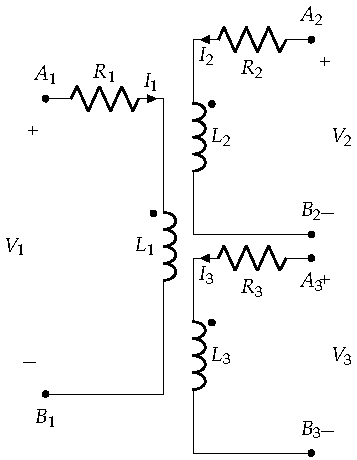
\includegraphics[height=0.25\textheight]{../figs/TrafoVariosDevanados.pdf}
  \caption{Representación circuital de un transformador real de varios devanados.}
  \label{fig:trafo-varios-devanados}
\end{figure}


Si aplicamos las condiciones de transformador perfecto (sección \ref{sec:trafo-perfecto}), la representación circuital es la de la figura \ref{fig:trafo-perfecto-varios-devanados} y las ecuaciones son:
  \begin{align*}
  \overline{U}_1 &= j \omega L_1 \cdot \overline{I}_1 + j \omega M_{12} \cdot\overline{I}_2 + j \omega M_{13} \cdot\overline{I}_3\\
  \overline{U}_2 &= j \omega M_{12} \cdot \overline{I}_1 + j \omega L_2 \cdot \overline{I}_2 + j \omega M_{23} \cdot \overline{I}_3\\
  \overline{U}_3 &= j \omega M_{13} \cdot \overline{I}_1 + j \omega M_{12} \cdot\overline{I}_2 + j \omega L_3 \cdot \overline{I}_3
\end{align*}

\begin{figure}
  \centering
  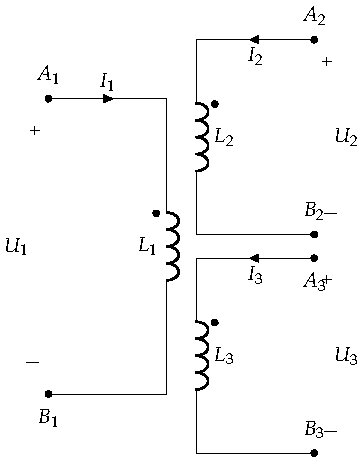
\includegraphics[height=0.25\textheight]{../figs/TrafoPerfectoVariosDevanados.pdf}
  \caption{Representación circuital de un transformador perfecto de varios devanados.}
  \label{fig:trafo-perfecto-varios-devanados}
\end{figure}

Si empleamos las relaciones de transformación de un transformador perfecto:
      \begin{align*}
  \frac{L_1}{L_2} &= \left(\frac{N_1}{N_2}\right)^2 = a^2_{12}\\
  \frac{L_1}{L_3} &= \left(\frac{N_1}{N_3}\right)^2 = a^2_{13}
\end{align*}
obtenemos las relaciones entre las tensiones de los devanados:
\begin{align}
  \frac{\overline{U}_1}{\overline{U}_2} &= a_{12}\\
  \frac{\overline{U}_1}{\overline{U}_3} &= a_{13}\label{eq:trafo-ideal-varios-devanados-tensiones}
\end{align}

Aplicando a continuación las condiciones de transformador ideal (sección \ref{sec:trafo-ideal}), las relaciones de corriente en el circuito de la figura \ref{fig:trafo-ideal-varios-devanados} son:
\begin{equation}
  \label{eq:trafo-ideal-varios-devanados-corrientes}
    N_1 \overline{I}_1 \pm N_ 2\overline{I}_2 \pm N_3
    \overline{I}_{3} = 0 \rightarrow
    \overline{I}_1 = \mp 1/a_{12} \cdot \overline{I}_2 \mp
    1/a_{13} \cdot \overline{I}_3
\end{equation}

\begin{figure}
  \centering
  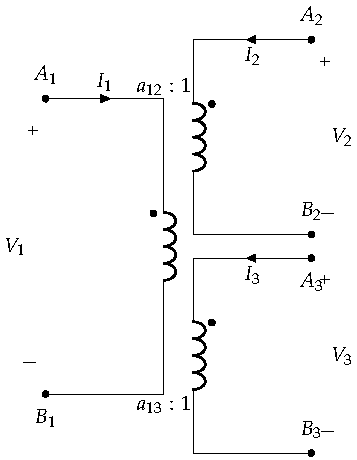
\includegraphics[height=0.25\textheight]{../figs/TrafoIdealVariosDevanados.pdf}
  \caption{Representación circuital de un transformador ideal de varios devanados.}
  \label{fig:trafo-ideal-varios-devanados}
\end{figure}

En la ecuación \ref{eq:trafo-ideal-varios-devanados-corrientes} emplearemos el signo positivo cuando las corrientes correspondientes tengan el mismo sentido y negativo con sentidos opuestos.

Con estas relaciones de tensiones y corrientes podemos obtener la impedancia equivalente vista desde un devanado de impedancias conectadas en los otros devanados (figura \ref{fig:trafo-ideal-varios-devanados-impedancia}). Las ecuaciones que corresponden a los devanados con impedancias son:
\begin{align*}
  \overline{U}_2 &= \overline{Z}_2 \cdot \overline{I}_2\\
  \overline{U}_3 &= \overline{Z}_3 \cdot \overline{I}_3
\end{align*}

\begin{figure}
  \centering
  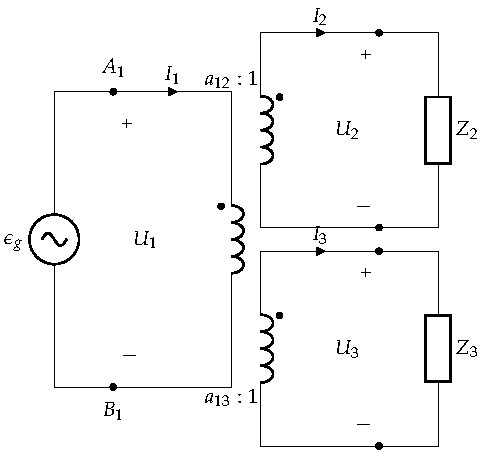
\includegraphics[height=0.25\textheight]{../figs/TrafoIdealVariosDevanados_Impedancia.pdf}
  \caption{Transformador ideal de varios devanados con una impedancia conectada en uno de ellos.}
  \label{fig:trafo-ideal-varios-devanados-impedancia}
\end{figure}

Combinando estas dos ecuaciones con las relaciones entre tensiones y corrientes (ecuaciones \ref{eq:trafo-ideal-varios-devanados-tensiones} y \ref{eq:trafo-ideal-varios-devanados-corrientes}) obtenemos la admitancia vista en el devanado sin carga. La ecuación \ref{eq:trafo-ideal-varios-devanados-impedancia} se puede interpretar como la admitancia equivalente de dos impedancias conectadas en paralelo y transferidas al devanado sin carga (figura \ref{fig:trafo-ideal-varios-devanados-impedancia-equivalente}).

\begin{equation}
  \label{eq:trafo-ideal-varios-devanados-impedancia}
  \overline{Y}_{in} = \frac{\overline{I}_1}{\overline{U}_1} = 
    \frac{1}{a^2_{12} \overline{Z}_2} + \frac{1}{a^2_{13}
      \overline{Z}_3}
\end{equation}

\begin{figure}
  \centering
  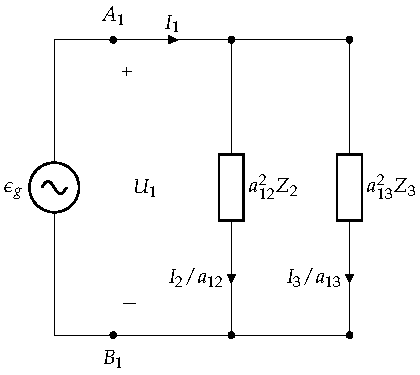
\includegraphics[height=.25\textheight]{../figs/TrafoIdealVariosDevanados_Impedancia_Equivalente.pdf}
  \caption{Circuito equivalente de un transformador ideal de tres devanados con impedancias conectadas en dos devanados.}
  \label{fig:trafo-ideal-varios-devanados-impedancia-equivalente}
\end{figure}
Ahora bien, ¿qué ocurre si el transformador no es ideal sino perfecto (figura \ref{fig:trafo-perfecto-varios-devanados-impedancia})? En este caso podemos sustituir el transformador perfecto por su equivalente de transformador ideal con una inductancia en paralelo (sección \ref{sec:perfecto-vs-ideal}), tal y como muestra la figura \ref{fig:trafo-perfecto-ideal-varios-devanados-impedancia}. En el circuito resultante podemos aplicar la relación obtenida en la ecuación \ref{eq:trafo-ideal-varios-devanados-impedancia} para concluir con el circuito equivalente de la figura \ref{fig:trafo-perfecto-ideal-varios-devanados-impedancia-equivalente}. En este circuito la inductancia del devanado sin carga está en paralelo con las impedancias de carga previamente transferidas a este devanado.

\begin{figure}
  \centering
  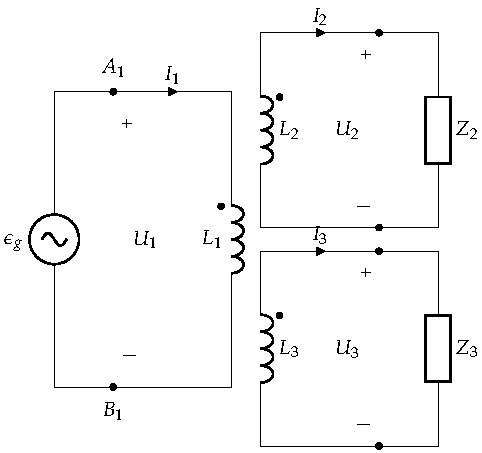
\includegraphics[height=0.25\textheight]{../figs/TrafoPerfectoVariosDevanados_Impedancia.pdf}
  \caption{Representación circuital de un transformador perfecto de tres devanados con impedancias conectadas en dos devanados.}
  \label{fig:trafo-perfecto-varios-devanados-impedancia}
\end{figure}
\begin{figure}
  \centering
  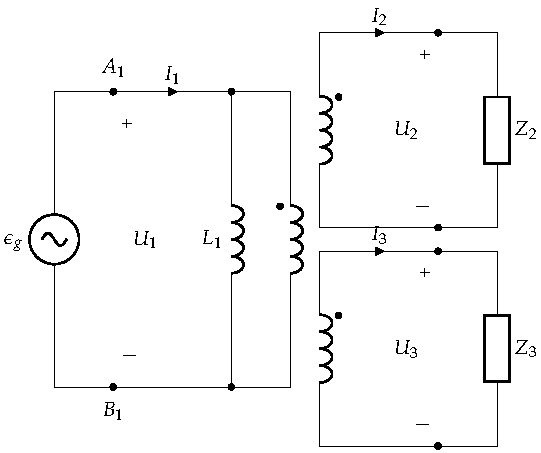
\includegraphics[height=0.25\textheight]{../figs/TrafoPerfectoIdealVariosDevanados_Impedancia.pdf}
  \caption{Representación circuital del transformador ideal equivalente de un transformador perfecto de tres devanados con impedancias conectadas en dos devanados.}
  \label{fig:trafo-perfecto-ideal-varios-devanados-impedancia}
\end{figure}
\begin{figure}
  \centering
  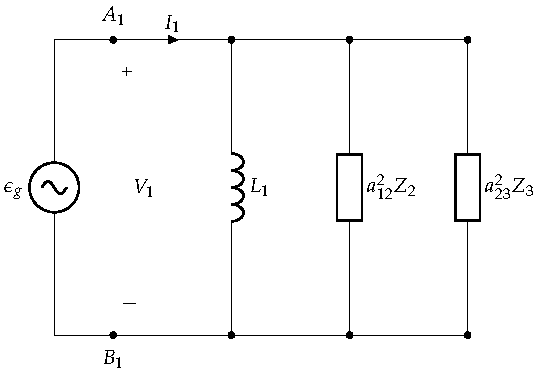
\includegraphics[height=0.25\textheight]{../figs/TrafoPerfectoVariosDevanados_Impedancia_Equivalente.pdf}
  \caption{Circuito equivalente de un transformador perfecto de tres devanados con impedancias conectadas en dos devanados.}
  \label{fig:trafo-perfecto-ideal-varios-devanados-impedancia-equivalente}
\end{figure}

\subsection{Autotransformador}
\label{sec:autotrafo}

Terminamos este capítulo con una sección dedicada al autotransformador. Este tipo de transformador posee un único devanado alrededor de un núcleo ferromagnético con tres terminales de conexión eléctrica (figura \ref{fig:autotrafo-perfecto}). Este tipo de transformador es más ligero que los anteriores, y permite regular la tensión de salida si el terminal intermedio es móvil. Sin embargo, el aislamiento galvánico que existía en los anteriores transformadores desaparece en esta configuración.

Las ecuaciones de un autotransformador perfecto son:
\begin{align*}
  \overline{U}_1 &= j \omega L_1 \cdot \overline{I}_1 + j \omega (M + L_2) \cdot \overline{I}_2\\
  \overline{U}_2 &= j \omega (M + L_2) \cdot \overline{I}_1 + j \omega L_2 \cdot \overline{I}_2
\end{align*}
siendo $M = \sqrt{L' \cdot L_2}$.

\begin{figure}\centering
  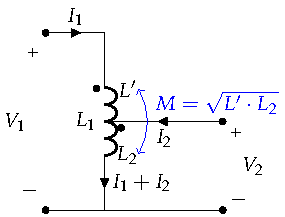
\includegraphics[height=0.25\textheight]{../figs/AutotrafoPerfecto.pdf}
  \caption{Representación circuital de un autotransformador perfecto.}
  \label{fig:autotrafo-perfecto}
\end{figure}

Una representación alternativa del autotransformador se muestra en la figura \ref{fig:autotrafo-perfecto2}, cuyas ecuaciones son:
\begin{align*}
  \overline{U}_1 &= j \omega (L' + L_2 + 2M) \cdot \overline{I}_1 + j \omega (L_2 + M) \cdot \overline{I}_2\\
  \overline{U}_2 &= j \omega (L_2 + M) \cdot \overline{I}_1 + j \omega L_2 \cdot \overline{I}_2
\end{align*}

\begin{figure}
  \centering
  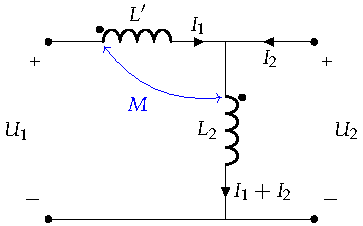
\includegraphics[height=0.25\textheight]{../figs/AutotrafoPerfecto2.pdf}
  \caption{Representación alternativa de un autotransformador perfecto.}
  \label{fig:autotrafo-perfecto2}
\end{figure}

Comparando las ecuaciones de ambas representaciones obtenemos la equivalencia $L_1 = L' + L_2 + 2M$. 
Además, en estas ecuaciones podemos observar que el término $L_2 + M$ juega el papel de coeficiente de inducción mutua entre los dos terminales. Así pues, si sustituimos este término por $M' = L_2 + M$ tendremos las ecuaciones de un transformador perfecto equivalente (figura \ref{fig:autotrafo-perfecto-equivalente}). Comprobemos que $M'$ es realmente el coeficiente de inducción mutua entre $L_1$ y $L_2$:
  \begin{align*}
  M' &= \sqrt{L_1 \cdot L_2} = \\
     &= \sqrt{(L' + L_2 + 2M) L_2} =\\
     &= \sqrt{L'L_2 + L_2^2 + 2ML_2} =\\
     &= \sqrt{M^2 + L_2^2 + 2ML_2} = \\
     &= M + L_2
\end{align*}
En consecuencia, podemos sustituir un autotransformador perfecto por un transformador perfecto respetando las relaciones:
\begin{align*}
  L_1 &= L' + L_2 + 2M\\
  M &= \sqrt{L' \cdot L_2}\\
  M' &= M + L_2
\end{align*}

\begin{figure}
  \centering
  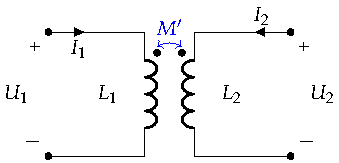
\includegraphics[height=0.2\textheight]{../figs/AutoTrafo_TrafoPerfecto.pdf}
  \caption{Transformador perfecto equivalente de un autotransformador perfecto.}
  \label{fig:autotrafo-perfecto-equivalente}
\end{figure}

En el caso de un autotransformador ideal (figura \ref{fig:autotrafo-ideal}), los terminales vendrán definidos por los números de vueltas de cada uno de ellos, $N_1$ y $N_2$. Así, la equivalencia es aún más sencilla, empleando únicamente la relación de transformación del transformador ideal $a = \frac{N_1}{N_2}$ (figura \ref{fig:autotrafo-ideal-equivalente}).

\begin{figure}
  \centering
  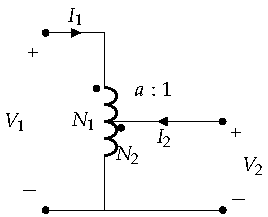
\includegraphics[height=.25\textheight]{../figs/AutoTrafoIdeal.pdf}
  \caption{Representación circuital de un autotransformador ideal.}
  \label{fig:autotrafo-ideal}
\end{figure}
\begin{figure}
  \centering
  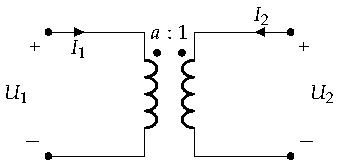
\includegraphics[height=.2\textheight]{../figs/Trafo_Ideal.pdf}
  \caption{Transformador ideal equivalente de un autotransformador ideal.}
  \label{fig:autotrafo-ideal-equivalente}
\end{figure}

%%% Local Variables:
%%% mode: latex
%%% TeX-master: "TC"
%%% ispell-local-dictionary: "castellano"
%%% End:
